\chapter{Simulations at negative temperatures}
\label{ch:ising}

In this last section I move the focus towards the study of a more complex model, namely the Ising model \cite{ising}. The higher complexity of the problem requires a numerical solution
via a Monte Carlo simulation. \\
After a brief introduction on the 2D Ising model, I will briefly recap the main points of a Markov Chain Monte Carlo algorithm, moving then towards the numerical experiments. The results of the
simulations are presented and discussed according to what said in the previous chapters. \\
\section{The Ising model}
\begin{figure}[htbp]
    \centering
    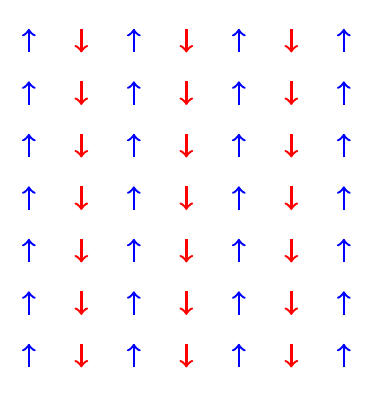
\begin{tikzpicture}
        \foreach \x in {-3,-1,1,3}{
        \foreach \y in {-3,-2,...,3}{
            \draw [->, line width=0.3mm, color=blue] (\x/1.5,\y/1.5-0.15) -- (\x/1.5,\y/1.5+0.15);
        }
      }
      \foreach \x in {-2,0,2}{
        \foreach \y in {-3,-2,...,3}{
            \draw [<-, line width=0.3mm, color=red] (\x/1.5,\y/1.5-0.15) -- (\x/1.5,\y/1.5+0.15);
        }
      }
    \end{tikzpicture}
    \caption{2D Ising model. The spins are organised in a 2D squared lattice and can assume only two values, either up or down. In the most general way the system is described by the Hamiltonian given by equation \ref{eq:general_Hamiltonian_Ising}}
    \label{fig:IsingLattice}
\end{figure}
The Ising model is a mathematical model initially used to describe magnetic properties of materials in statistical mechanics. It consists of a collection of spins 
organised in a lattice that can assume two values, either 1 or -1. \\
The spins are allowed to interact with their nearest neighbors and in the most general form the Hamiltonian assumes the form
\begin{equation}
    \mathcal{H}(\{\sigma_k\}) = -\sum_{\langle i j\rangle} J_{i j} \sigma_{i} \sigma_{j} - \sum_{j} B_j\sigma_{j}
    \label{eq:general_Hamiltonian_Ising}
\end{equation}
where $B_j$ indicates the intensity of the magnetic field on the spin $j$ and $J_{ij}$ indicates the strength of the interaction between the spin $i$ and the spin $j$.
In the following analysis I will assume $J_{ij} = J, B_j = B \ \forall i,j$. \\
The sign of the interaction parameter $J$ determines whether we are dealing with ferromagnetic materials ($J>0$) or antiferromagnetic materials ($J < 0$). In the case of $J=0$
we return to the two levels system discussed in chapter \ref{ch:TLS}. \\
Let us first restrict the analysis to the purely interacting case setting $B=0$. In this case the Hamiltonian initially given by \ref{eq:general_Hamiltonian_Ising} becomes
\begin{equation*}
    \mathcal{H}(\{\sigma_k\}) = -J \sum_{\langle i j\rangle}\sigma_{i} \sigma_{j}
\end{equation*}
At fixed temperature $T$ the probability of a state is given by the Boltzmann factor
\begin{equation}
    p(\{\sigma_k\}) = \frac{e^{-\beta\mathcal{H}(\{\sigma_k\})}}{Z}
    \label{eq:Boltzmann_factor_Ising}
\end{equation}
where $\beta = \frac{1}{k_BT}$ and $Z$ is the canonical partition function
\begin{equation*}
    Z(\beta, B, N) = \sum_{\{\sigma_k\}} e^{-\beta\mathcal{H}(\{\sigma_k\})}
\end{equation*}
Let us consider the probability factor \ref{eq:Boltzmann_factor_Ising}, which explicitly becomes 
\begin{equation*}
    p(\{\sigma_k\}) \propto e^{\beta J \sum_{\langle i j\rangle}\sigma_{i} \sigma_{j}}
\end{equation*}
and let us define a new parameter $\xi = \beta J$ so that 
\begin{equation}
    p(\{\sigma_k\}) \propto e^{\xi \sum_{\langle i j\rangle}\sigma_{i} \sigma_{j}}
    \label{eq:probability_Ising}
\end{equation}

\subsection{Ferromagnetic systems}
\label{subsec:ferromagnetic}
In the ferromagnetic case $J > 0$, hence $\xi > 0$. 
\begin{itemize}
    \item For $\xi \to 0$, which can be either a high temperature or a weak coupling, one can see that 
    $p(\{\sigma_k\}) \to 1$ independently of the values $\sigma_k$ so that every distribution $\{\sigma_k\}$ is equally probable.
    Thus, macroscopically speaking, we expect the system to be found in a \emph{disordered} state.
    \item When $\xi \to +\infty$ the exponential factor in \ref{eq:probability_Ising} grows indefinetely if $\sum_{\langle i j\rangle}\sigma_{i} \sigma_{j} > 0$, that is when the spins are aligned.
    We then expect the system to be in a \emph{highly ordered} configuration organised into clusters of spins aligned in the same direction.
    Thus no preference is given to the configuration in which spins are aligned both up or down, and we expect it to depend on the history of the system. \\
\end{itemize}
\subsection{Antiferromagnetic systems}
\label{subsec:antiferromagnetic}
In this case $J < 0$, hence $\xi < 0$. 
\begin{itemize}
    \item For $\xi \to 0$ the result is the same of ferromagnetic systems.
    \item On the other side for $\xi \to -\infty$, which can be either a low temperature or a strong coupling, one can see that 
    $p(\{\sigma_k\}) \to 0$ except when $\sum_{\langle i j\rangle}\sigma_{i} \sigma_{j} = 0$, that is when neighbour spins are disaligned. We then expect the system to be found in an \emph{ordered configuration} in which 
    neighbor spins are disaligned.
\end{itemize}
The study is carried in a 2D lattice which is of the shape reported in figure \ref{fig:IsingLattice}.
Let us focus the attention on a $2\times2$ subset of the lattice and let us consider $J>0$ as an example. The possible energies are 
\begin{align*}
    \begin{pmatrix} \uparrow & \uparrow \\ \uparrow & \uparrow \end{pmatrix},&
    \begin{pmatrix} \downarrow & \downarrow \\ \downarrow & \downarrow \end{pmatrix} \qquad \qquad &E = -4J \\
    \begin{pmatrix} \downarrow & \uparrow \\ \uparrow & \uparrow \end{pmatrix}, \,
    \begin{pmatrix} \uparrow & \downarrow \\ \uparrow & \uparrow \end{pmatrix},& \,
    \begin{pmatrix} \uparrow & \uparrow \\ \downarrow & \uparrow \end{pmatrix}, \,
    \begin{pmatrix} \uparrow & \uparrow \\ \uparrow & \downarrow \end{pmatrix} \qquad &E = 0J \\
    \begin{pmatrix} \downarrow & \downarrow \\ \uparrow & \uparrow \end{pmatrix}, \,
    \begin{pmatrix} \downarrow & \uparrow \\ \downarrow & \uparrow \end{pmatrix}, \, &
    \begin{pmatrix} \uparrow & \downarrow \\ \uparrow & \downarrow \end{pmatrix}, \,
    \begin{pmatrix} \uparrow & \uparrow \\ \downarrow & \downarrow \end{pmatrix} \qquad &E = 0J \\
    \begin{pmatrix} \uparrow & \downarrow \\ \downarrow & \downarrow \end{pmatrix}, \,
    \begin{pmatrix} \downarrow & \uparrow \\ \downarrow & \downarrow \end{pmatrix}, \,&
    \begin{pmatrix} \downarrow & \downarrow \\ \uparrow & \downarrow \end{pmatrix}, \,
    \begin{pmatrix} \downarrow & \downarrow \\ \downarrow & \uparrow \end{pmatrix} \qquad &E = 0J \\
    \begin{pmatrix} \downarrow & \uparrow \\ \uparrow & \downarrow \end{pmatrix},& \,
    \begin{pmatrix} \uparrow & \downarrow \\ \downarrow & \uparrow \end{pmatrix}, \qquad &E = 4J \\
\end{align*}
The whole system is then a repetition of these blocks and the total energy of the system is the sum of the energies of each block. One can observe 
that 
\begin{enumerate}
    \item The lowest energy configuration is the one with all the spins aligned either up or down as predicted previously.
    \item The highest energy configuration corresponds to the lowest energy configuration of the antiferromagnetic case according to what predicted previously. I will show later that this 
    is explained if the ferromagnetic system is described by a negative temperature, more precisely $T = -\SI{0}{\kelvin}$.
    \item The number of states at energy given energy $E$ is equal to the number of states at energy $-E$. This means that the density of states function $\omega(E)$ is an even function 
    of the energy, that is $\omega(E) = \omega(-E)$. Remembering that the derivative of a continuous even function is an odd function, one has that the temperature function
    \begin{equation*}
        \frac{1}{T} = \frac{\partial S}{\partial E} = k_B \frac{\omega'(E)}{\omega(E)}
    \end{equation*}
    is an odd function of the energy, hence proving that the described model admits negative temperatures. Since the maximum point for $\omega(E)$ is expected for $E=0$, $\omega'(E)$ is negative for $E>0$,
    suggesting that negative temperatures describe high energy configurations of the system.
\end{enumerate}
In what follows I will adopt the so called \emph{free boundary conditions}, which means not putting any constraints on the spins at the boundary of the system.

\section{Markov Chain Monte Carlo}
\label{sec:MCMC}
To study the physical properties of the system at equilibrium in a certain macrostate $X$, one needs to perform ensemble averages (or expectation values). The expectation value of a physical quantity $A$ is computed as 
\begin{equation}
    \bar A = \frac{\int A e^{-\beta H} d\tau}{\int e^{-\beta H} d \tau}
    \label{eq:averageval}
\end{equation}
where tha variable $\tau$ runs over all the possible microstates compatible with the given macrostate $X$. \\
Practically speaking, to perform such averages during the simulation, one needs to
\begin{enumerate}
    \item Bring the system in a configuration compatible with the specified macrostate 
    \item Calculate the value of the desired quantity in the specific microstate and store the value
    \item Move the system to another microstate compatible with the specified macrostate and repeat from point 2 until desired
    \item Perform the average
\end{enumerate}
Of course, in order to perform an accurate average, one needs to 
\begin{enumerate}
    \item Guarantee that the system visits every possible microstate compatible with the macroscopical configuration so that all the possible values of the physical quantity are taken into account when performing the average
    \item Guarantee that every possible state is visited with a frequency that is equal to the probability of the state itself
\end{enumerate}
This can be accomplished with a Monte Carlo method, precisely by means of the \emph{Metropolis-Hastings algorithm}, which allows one to perform a random walk trough the configurations of the system and respect the above stated conditions. \\
The main points of the Metropolis-Hastings' \cite{Hastings} algorithm are now briefly reported, inviting the reader to consult more appropriate sources for further information. \par
\vspace{10pt}
Let us suppose that we want to sample from a probability distribution $p(x)$. \\
The system is initially prepared in a certain configuration $x$ which can be arbitrarilly chosen. Each Monte-Carlo cycle then consists in the following steps
\begin{enumerate}
    \item A new configuration of the system $x^*$ is proposed sampling from a proposal distribution $J(x^*|x_i)$. The proposal distribution can be arbitrarilly chosen, provided the fact that it is symmetric $J(x^*|x_i) = J(x_i|x^*)$
    \footnote{Strictly speaking this is the simple Metropolis algorithm. The more general Metropolis-Hastings algorithm does not need the proposal distribution to be symmetric, provided the probability ratio $w$ is modified to $w=\frac{J(x_i|x^*)p(x^*)}{J(x^*|x_i)p(x_i)}$.}
    and that in an infinite number of steps, it guarantees that every state is visited.
    \item The ratio of the probabilities of the two states of the system is then calculated
    \begin{equation*}
        w = \frac{p(x^*)}{p(x_i)}
    \end{equation*}
    \item if $w \geq 1$ the proposal change is accepted and $x_{i+1} = x^*$
    \item otherwise a number $r$ is extracted from a uniform distribution in $[0,1]$. If $w > r$ the proposal change is still accepted and $x_{i+1} = x^*$. Otherwise the proposal moved is refused and $x_{i+1} = x_i$
\end{enumerate}
The higher the number of Monte Carlo cycles, the closer the distribution of the visited states to the probability distribution $p(x)$, the more precise the expectation values calculated as \ref{eq:averageval}. \\
The simplest choice for the proposal distribution $J(x^*|x)$, even if not the most efficient, is the uniform distribution. The distribution $p(x)$, on the other side, is related to the ensemble 
in which we describe the system: in the canonical ensemble $p(x)$ is given by the Maxwell-Boltzmann distribution given by equation \ref{eq:Boltzmann_factor_Ising}.
\newpage

\section{Single system at negative temperature}
The first case I want to study is the equilibirum configuration of one single system prepared at a given temperature $T$. After fixing the temperature, the system is prepared in a random configuration: then the system goes under $10^6$ Monte Carlo cycles 
sampling from the probability distribution given by \ref{eq:Boltzmann_factor_Ising}. An example of initial configuration is reported in figure \ref{fig:initial_configuration}. \par
\begin{figure}[htp]
    \centering 
    \centering
    \includegraphics[scale=0.6]{./images/ising/initconf.eps}
    \caption{Initial configuration for the system. Each spin value was extracted randomly between $+1$ or $-1$. A blue tile indicates an up spin, while a white one indicates a down spin.}
    \label{fig:initial_configuration}
\end{figure}
The simulations are run for four different values of temperature, that is 
\begin{equation*}
    T_1 = \SI{0.01}{\kelvin} \qquad T_2 = \SI{-0.01}{\kelvin} \qquad T_3 = \SI{100}{\kelvin} \qquad T_4 = \SI{-100}{\kelvin}
\end{equation*}
Each of them is run both for the ferromagnetic and antiferromagnetic cases. \\
Figure \ref{fig:MC_single_final_state_ferro} reports the final states of a ferromagnetic system, while
figure \ref{fig:MC_single_final_state_antiferro} reports those of an antiferromagnetic system.\\
\begin{figure}[ht]
    \begin{subfigure}{.45\textwidth}
        \centering
        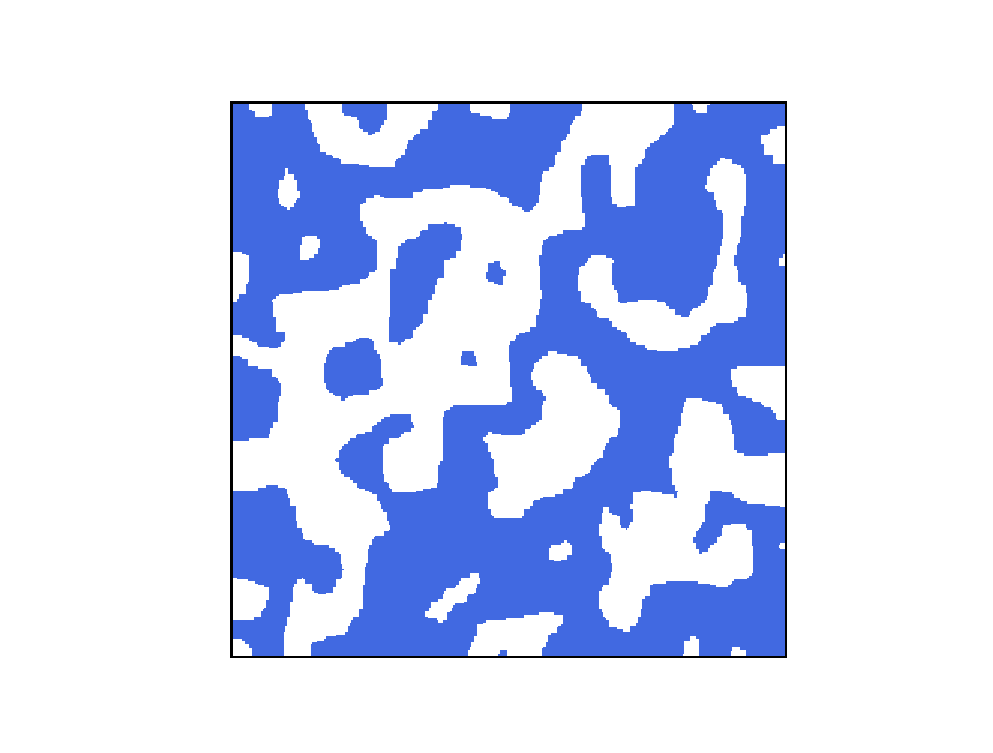
\includegraphics[width=200px]{./images/ising/T_001_ferro.eps}
        \caption*{$T = \SI{0.01}{\kelvin}$}
    \end{subfigure}
    \begin{subfigure}{.45\textwidth}
        \centering
        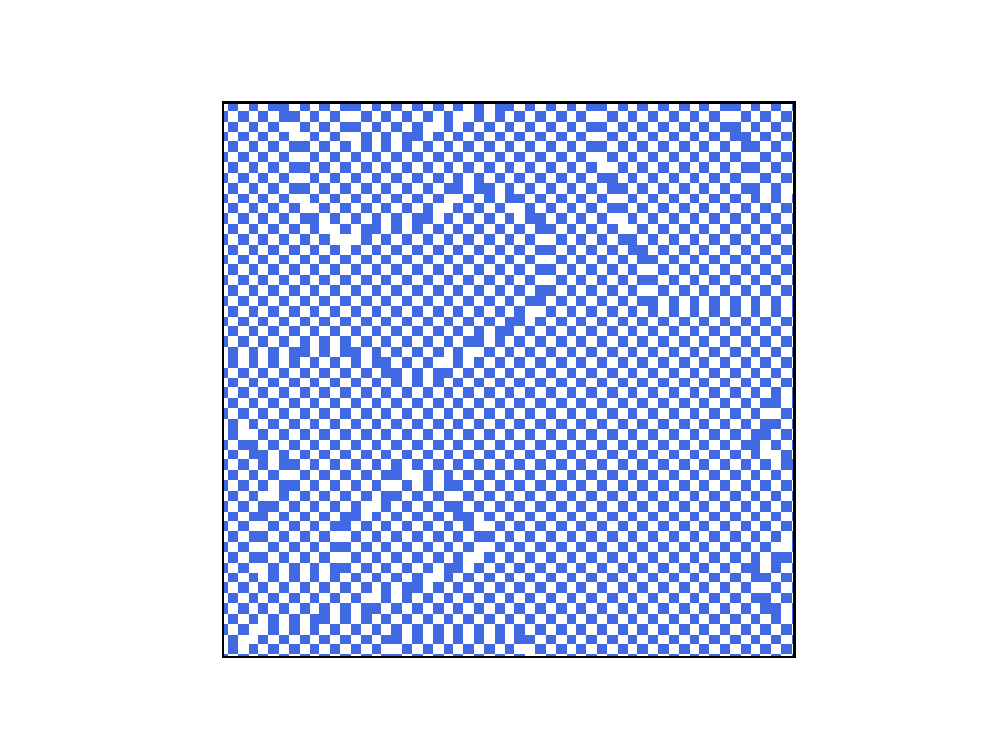
\includegraphics[width=200px]{./images/ising/T_n001_ferro.eps}
        \caption*{\hspace{20pt} $T = \SI{-0.01}{\kelvin}$ (zoomed)}
    \end{subfigure}
    \newline
    \begin{subfigure}{.45\textwidth}
        \centering
        \includegraphics[width=200px]{./images/ising/T_100_ferro.eps}
        \caption*{$T = \SI{100}{\kelvin}$}
    \end{subfigure}
    \begin{subfigure}{.45\textwidth}
        \centering
        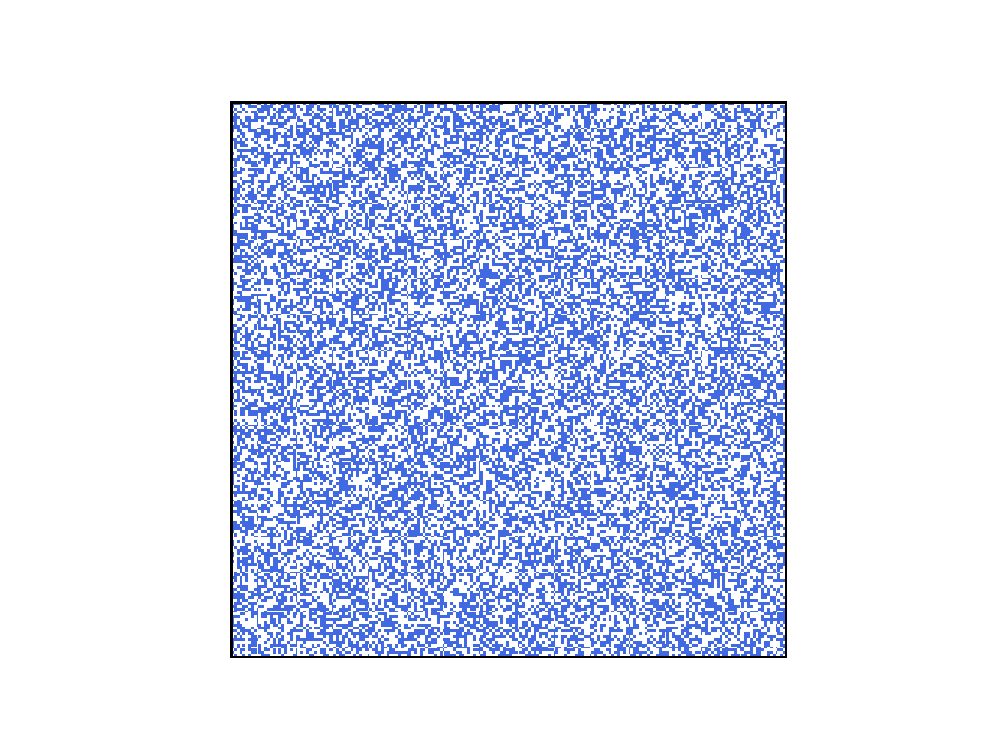
\includegraphics[width=200px]{./images/ising/T_n100_ferro.eps}
        \caption*{$T = \SI{-100}{\kelvin}$}
    \end{subfigure}
    \caption{Ferromagnetic system}
    \label{fig:MC_single_final_state_ferro}
\end{figure}
\begin{figure}[ht]
    \begin{subfigure}{.45\textwidth}
        \centering
        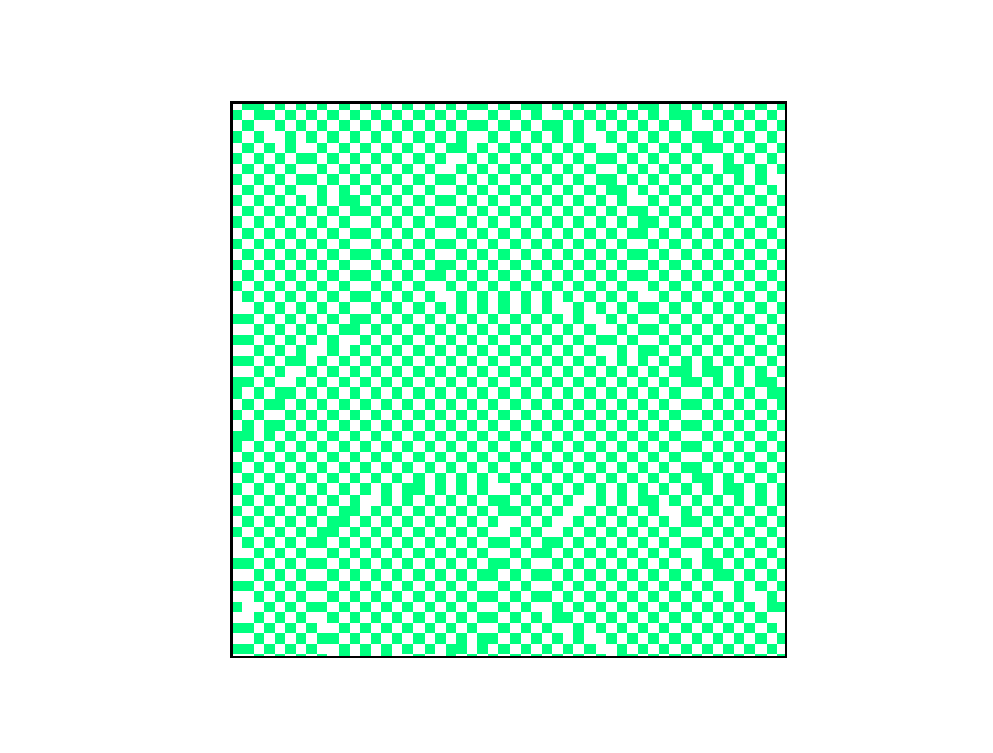
\includegraphics[width=200px]{./images/ising/T_001_antiferro.eps}
        \caption*{\hspace{20pt} $T = \SI{0.01}{\kelvin}$ (zoomed)}
    \end{subfigure}
    \begin{subfigure}{.45\textwidth}
        \centering
        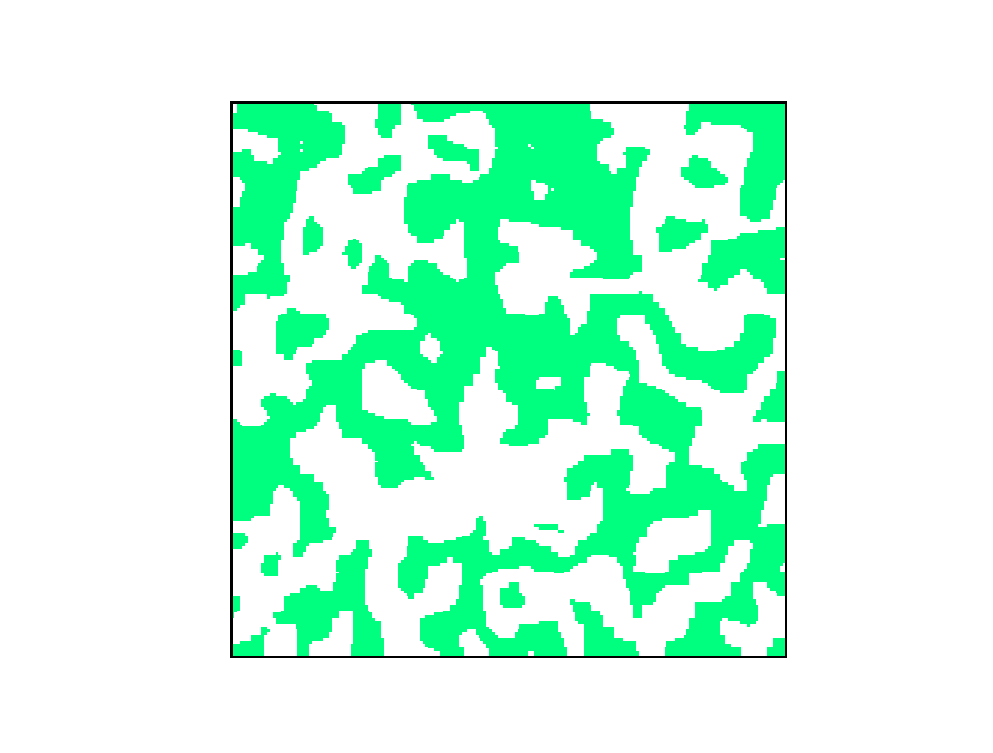
\includegraphics[width=200px]{./images/ising/T_n001_antiferro.eps}
        \caption*{$T = \SI{-0.01}{\kelvin}$}
    \end{subfigure}
    \newline
    \begin{subfigure}{.45\textwidth}
        \centering
        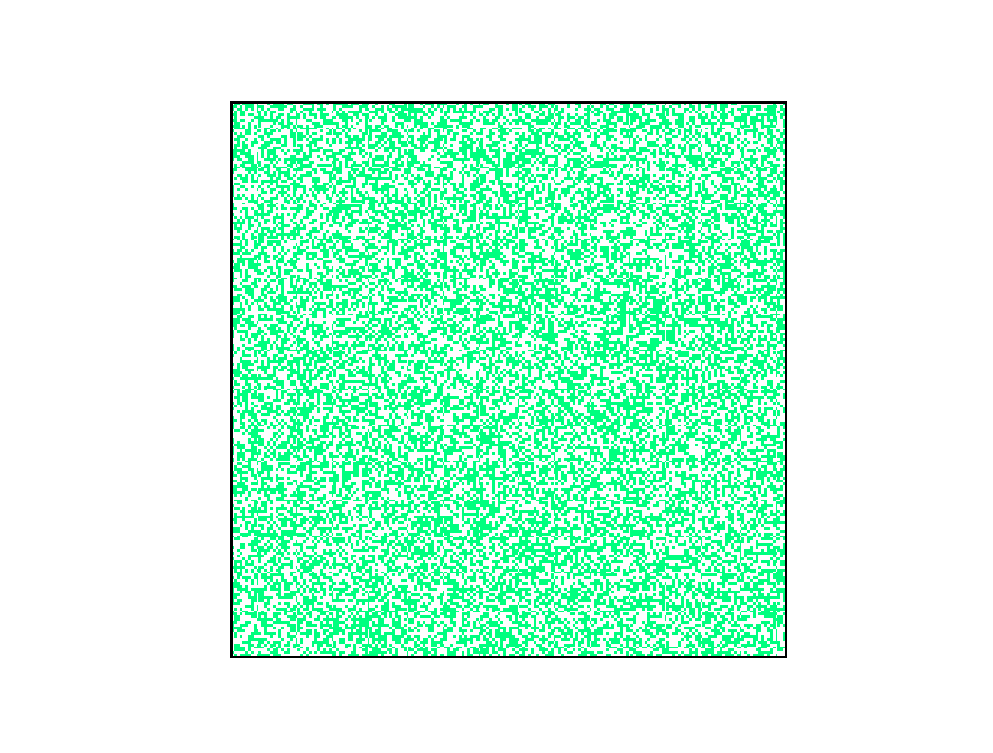
\includegraphics[width=200px]{./images/ising/T_100_antiferro.eps}
        \caption*{$T = \SI{100}{\kelvin}$}
    \end{subfigure}
    \begin{subfigure}{.45\textwidth}
        \centering
        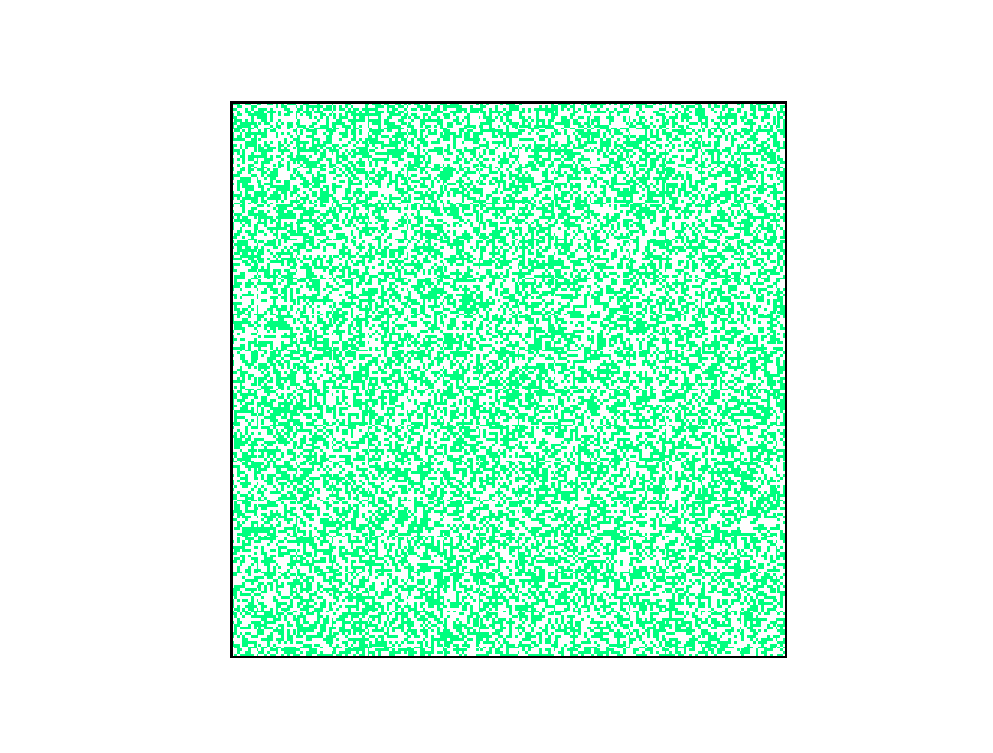
\includegraphics[width=200px]{./images/ising/T_n100_antiferro.eps}
        \caption*{$T = \SI{-100}{\kelvin}$}
    \end{subfigure}
    \caption{Antiferromagnetic system}
    \label{fig:MC_single_final_state_antiferro}
\end{figure}
According to what predicted in paragraph \ref{subsec:ferromagnetic}, at low positive temperature the system tends to organize
in an ordered structure grouping the spins into bigger clusters. As the temperature increases, the system starts forming imperfections increasing its disorder. This can be understood 
also in terms of the minimal free energy principle. In the canonical ensemble the most probable configuration is the one that minimizes the free energy
\begin{equation}
    F(T, V) = E - TS
    \label{eq:free_energy}
\end{equation}
which is the Legendre transform of the internal energy $E(S, V) = TS - PV$ with respect to the conjugate variables $T \leftrightarrow S$. The free energy minimization at fixed temperature, according to the definition \ref{eq:free_energy},
can be driven either by the minimization of the internal energy or by an increase in the entropy. The higher the temperature, the higher the entropic contribution, hence explaining why 
we find a disordered configuration at high temperature. \par
\vspace{10pt}
As for the ferromagnetic case, the results for the antiferromagnetic system agree with what predicted in section \ref{subsec:antiferromagnetic}. For high temperature the free energy minimazion is driven by the entropic contribute, leading to a high disordered configuration. 
For low positive temperature the minimization of the energy 
\begin{equation*}
    \mathcal{H}(\{\sigma_k\}) = -J \sum_{\langle i j\rangle}\sigma_{i} \sigma_{j}
\end{equation*}
requires the spins to be disaligned in couples, thus leading to a configuration in which neighbor spins alternate between up and down. \par
\vspace{10pt}
The result for negative temperatures can be easilly interpreted by looking at the definition of $\xi = \beta J$. All the result I discussed in this chapter made use of the value and the sign of $\xi$ but no specifications were made on whether the global sign came from $\beta$ or $J$ (see sections \ref{subsec:ferromagnetic} and \ref{subsec:antiferromagnetic}). A negative sign on $\xi$ can in fact be attributed either to 
a negative $\beta$ and a positive $J$, or vice versa. For example for $J>0$ (ferromagnetic) and temperature $T<0$ one has that $\xi < 0$ but the sign can be "moved" to $J$ suggesting a formal switch to the antiferromagnetic case with temperature $-T$. In formulas, for $\beta < 0$ and $J > 0$
\begin{equation*}
    0 > \xi = \beta J = -|\beta| J = |\beta| (-J)
\end{equation*}
Indeed it can be seen comparing figure \ref{fig:MC_single_final_state_ferro} with \ref{fig:MC_single_final_state_antiferro} that the result for $T = \SI{0.01}{\kelvin}$ ($-\SI{0.01}{\kelvin}$) in the ferromagnetic case corresponds to the one for $T = - \SI{0.01}{\kelvin}$ ($\SI{0.01}{\kelvin}$) in the antiferromagnetic case. \\
One can explain the similarity between the cases $T = \SI{100}{\kelvin}$ and $T = \SI{-100}{\kelvin}$ by noting that the limit $T \to \pm \infty$ corresponds to $\beta \to 0$ independently of the sign of the temperature, and $\beta$ is the parameter that determines the physical behaviour since it is the one that enters in the probability factor \ref{eq:Boltzmann_factor_Ising}.

\section{Two systems into contact}
The second simulation consists in preparing two systems at different temperatures, one of which is negative, and putting them into contact, observing the behaviour of the two systems at equilibrium. \\
The physical content of the experiment is better appreciated if we return to the non-interacting case of the two levels system and we use the Hamiltonian
\begin{equation*}
    \mathcal{H}(\{\sigma_k\}) = -B \sum_i \sigma_i
\end{equation*}
The first system is prepared at temperature $T_1 = \SI{-0.01}{\kelvin}$, and since $\frac{1}{T} = \frac{\partial S}{\partial E}$, the system lies on the right edge of the plot in figure \ref{eq:TLS_ensemble_energy}, that is the configuration with maximal energy with all the spins aligned antiparallel with respect to the field. This can 
also be seen by looking at the Boltzmann probability factor.
\begin{equation*}
    p(\{\sigma_k\}) = e^{-|\beta| B \sum_i \sigma_i}
\end{equation*}
which, for small $\beta$, is maximal when $\sum_i \sigma_i$ is miminal (most negative), that is when all the spins are aligned antiparallel with respect to the field.
The second system is prepared at temperature $T=\SI{100}{\kelvin}$ and corresponds to a highly disordered configuration, since for $\beta \to 0$ the Boltzmann factor goes to $1$ independently of the values $\sigma_i$, meaning that all the microscopic configurations are equally probable. \paragraph{}
Each system is a $200 \times 200$ squared lattice. Again, I choose the free boundary conditions. Each system goes under $10^6$ Monte Carlo steps in order to bring them in thermal equilibrium. The configurations of the systems before contact are reported in figure \ref{fig:contact_initial}. \par
\begin{figure}[hbtp]
    \hfill
    \begin{minipage}[c]{0.45\textwidth}
        \centering 
        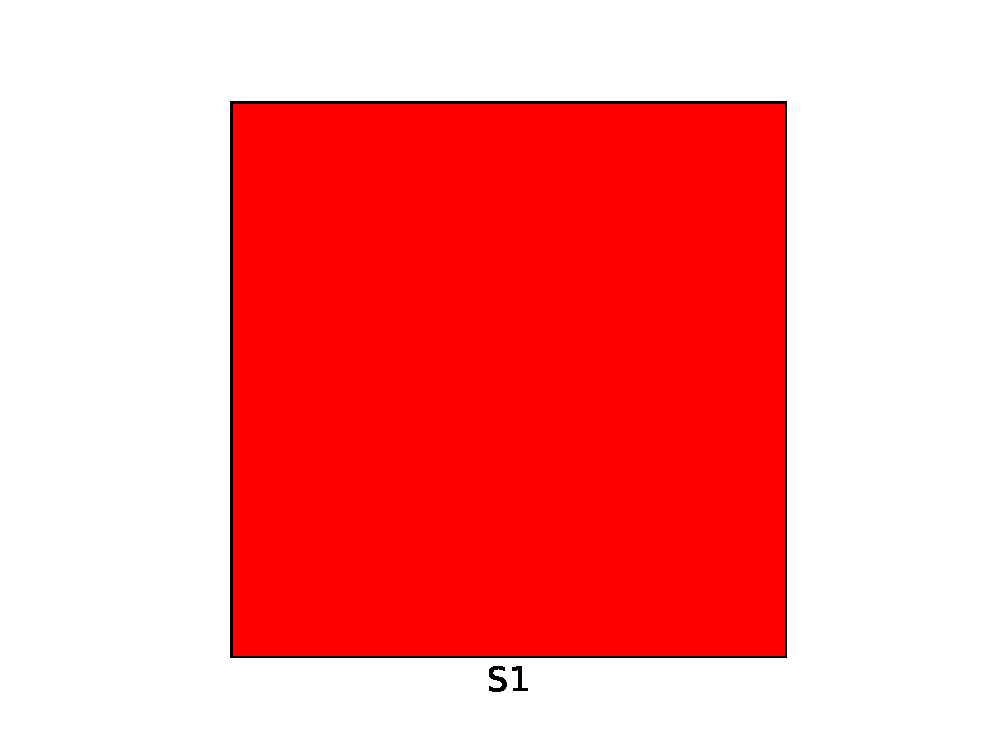
\includegraphics[scale=0.45]{images/ising/mixing_S1_before}
    \end{minipage}
    \hfill
    \begin{minipage}[c]{0.45\textwidth}
        \centering 
        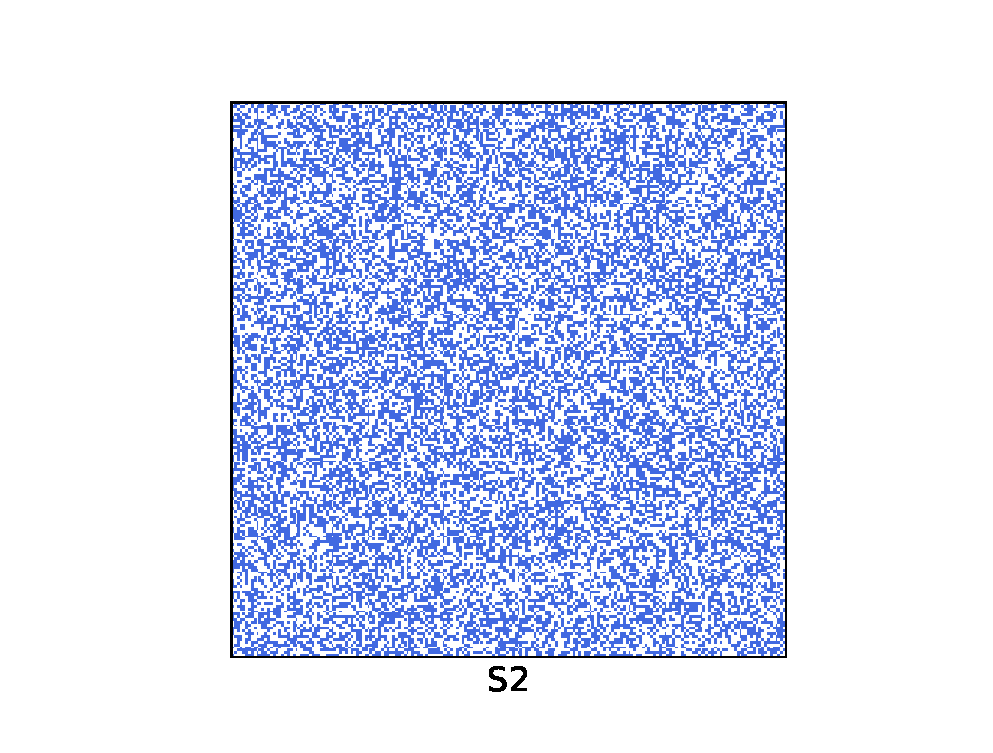
\includegraphics[scale=0.45]{images/ising/mixing_S2_before}
    \end{minipage}
    \hfill
    \caption{The figure reports the configurations of the systems $\mathcal{S}_1$ and $\mathcal{S}_2$ after thermalization. The systems $\mathcal{S}_1$ and $\mathcal{S}_2$ are prepared respectively at temperatures $T_1 = \SI{-0.01}{\kelvin}$ and $T_2 = \SI{100}{\kelvin}$. A blue tile indicates an up spin, while a white one indicates a down spin.}
    \label{fig:contact_initial}
\end{figure}
\vspace{10pt}
\begin{figure}[htbp]
    \centering
    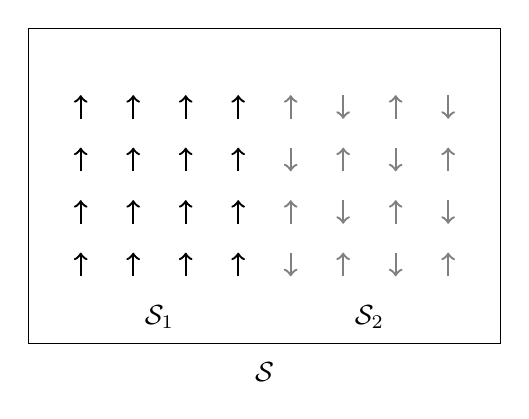
\begin{tikzpicture}
        \foreach \x in {-3,...,0}{
            \foreach \y in {-2,...,1}{
                    \draw [->, color=black!100, line width=0.3mm] (\x/1.5,\y/1.5-0.15) -- (\x/1.5,\y/1.5+0.15);
                }
            }
        \foreach \y in {-1,1}{
            \foreach \x in {1,3}{
                \draw [->, color=black!50, line width=0.3mm] (\x/1.5,\y/1.5-0.15) -- (\x/1.5,\y/1.5+0.15);
            }
            \foreach \x in {2,4}{
                \draw [<-, color=black!50, line width=0.3mm] (\x/1.5,\y/1.5-0.15) -- (\x/1.5,\y/1.5+0.15);
            }
        }
        \foreach \y in {-2,0}{
            \foreach \x in {1,3}{
                \draw [<-, color=black!50, line width=0.3mm] (\x/1.5,\y/1.5-0.15) -- (\x/1.5,\y/1.5+0.15);
            }
            \foreach \x in {2,4}{
                \draw [->, color=black!50, line width=0.3mm] (\x/1.5,\y/1.5-0.15) -- (\x/1.5,\y/1.5+0.15);
            }
        }
        \draw (-4/1.5,-3.5/1.5) -- (-4/1.5,2.5/1.5) -- (5/1.5,2.5/1.5) -- (5/1.5,-3.5/1.5) -- (-4/1.5,-3.5/1.5);
        \node[align=left] at (-1,-2) {$\mathcal{S}_1$};
        \node[align=left] at (2.5/1.5,-2) {$\mathcal{S}_2$};
        \node[align=left] at (0.5/1.5,-2.7) {$\mathcal{S}$};
    \end{tikzpicture}
    \caption{The systems $\mathcal{S}_1$ and $\mathcal{S}_2$, prepared at temperatures $T_1$ and $T_2$, are put into contact forming a new system $\mathcal{S}$ of $2N \times N$ sites (the figure is shown transposed).}
    \label{fig:contact_symbolized}
\end{figure}
The systems are then brought into contact: this is done pratically by creating a $400 \times 200$ lattice and copying the values of the two separated systems into the new one. The system is initialized 
with energy $E = E_1 + E_2$ where the the two energies refers to the energies of the systems $\mathcal{S}_1$ and $\mathcal{S}_2$ before putting them into contact. The study then proceeds in the microcanonical ensemble 
with energy $E$, trying to search the configuration that maximizes the entropy given the available energy. The algorithm used for the simulation is not exactly the one introduced in section \ref{sec:MCMC} but the so called \emph{demon Monte Carlo}, which can be summarized in the following steps. \\
At first, a new degree of freedom is introduced in the system, called the demon. The demon energy must be positive but there are no restrictions on the upper value. Then
\begin{enumerate}
    \item Propose the new state for the system as explained in section \ref{sec:MCMC}
    \item Calculate the energy difference between the two states
    \item If $\Delta E < 0$ the proposal is accepted and the demon takes the energy excess
    \item If $\Delta E > 0$ but it is smaller than the demon's energy, the demon releases his energy and the move is accepted. Otherwise the move is rejected.
    \item Repeat from point 1
\end{enumerate}
The higher the number of degrees of freedom in the system, the less the demon contribution to the energy of the system, the better energy can be considered conserved in the true degrees of freedom of the system. \\
After $10^7$ Monte Carlo cycles, the configuration is reported in figure \ref{fig:contact_final}, for convenience splitted again into the two subsystems.
\begin{figure}[hbtp]
    \hfill
    \begin{minipage}[c]{0.45\textwidth}
        \centering 
        \includegraphics*[scale=0.45]{images/ising/mixing_S1_after}
    \end{minipage}
    \hfill
    \begin{minipage}[c]{0.45\textwidth}
        \centering 
        \includegraphics*[scale=0.45]{images/ising/mixing_S2_after}
    \end{minipage}
    \hfill
    \caption{The figure reports the configurations of the systems $\mathcal{S}_1$ and $\mathcal{S}_2$ after beeing put into contact. After a thermalization of $10^7$ Monte Carlo steps, the two systems must share the same temperature as by definition of equilibrium. \\
    As before, a blue tile indicates an up spin, while a white one indicates a down spin.}
    \label{fig:contact_final}
\end{figure}
It can be seen that in the final state of the two systems there is a prevalence of up spins rather than downs due to energy conservation in the process of putting $\mathcal{S}_1$ and $\mathcal{S}_2$ into contact. The system $\mathcal{S}_1$, initially prepared at temperature $T_1 = \SI{-0.01}{\kelvin}$ with almost all the spins up, at equilibrium has reduced his number of up spins, still
beeing in a configuration of inverted population: this means that its temperature has decreased passing to a more negative one. The heat was transferred to the system $\mathcal{S}_2$, who passed from a high positive temperature to a negative one. The total energy of the system $E = E_1 + E_2$ is then equally splitted between $\mathcal{S}_1$ and $\mathcal{S}_2$. The situation is resumed in figure \ref{fig:contact_E_S_1}
\begin{figure}[h!]
    \centering 
    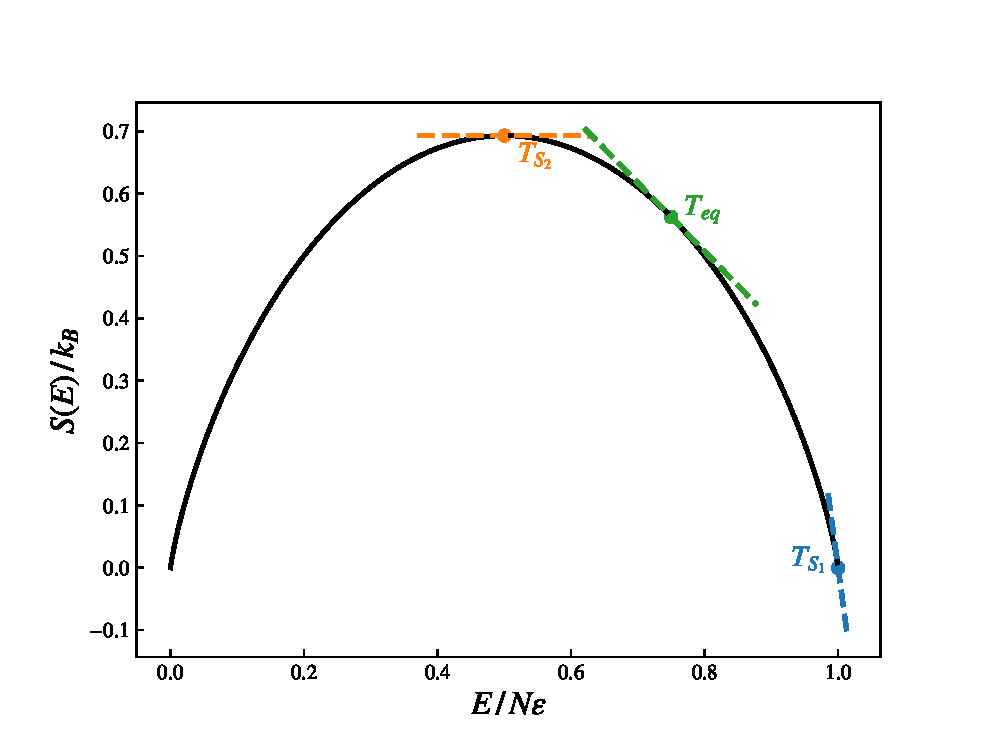
\includegraphics[scale=0.6]{./images/ising/mixing_SE_plot.eps}
    \caption{The plot resumes the configurations of the systems $\mathcal{S}_1$ and $\mathcal{S}_2$ before and after putting them into conctact. The system $\mathcal{S}_1$ is prepared at $T = \SI{-0.01}{\kelvin}$ in a high energy configuration (blue point in the plot), while $\mathcal{S}_2$ is prepared at temperature $T = \SI{100}{\kelvin}$ (orange point in the plot). After allowing the contact, 
    $\mathcal{S}_1$ releases heat to $\mathcal{S}_2$, splitting the total energy $E = E_1 + E_2$ equally between the two systems. At equilibrium $\mathcal{S}_1$ and $\mathcal{S}_2$ lie at the same temperature $T_{eq}$, with the same energy $E = \frac{E_1 + E_2}{2}$}
    \label{fig:contact_E_S_1}
\end{figure}